\documentclass[letterpaper,headings=standardclasses]{scrartcl}

\usepackage[margin=1in,includefoot]{geometry}
\usepackage{amssymb}
\usepackage{amsmath}
\usepackage{listings}
\usepackage{tikz}

\usetikzlibrary{shapes,arrows}

\tikzset{
  block/.style    = {draw, thick, rectangle, minimum height = 3em, minimum width = 3em},
  sum/.style      = {draw, circle, node distance = 2cm},
  input/.style    = {coordinate, circle},
  output/.style   = {coordinate, circle}
}

\lstset{basicstyle=\ttfamily,columns=flexible,breaklines=true}

\title{Homework 1}
\subtitle{CS 559 - Neural Networks - Fall 2019}
\author{Matteo Corain 650088272}

\begin{document}

\maketitle

\section{Question 1}

\subsection{First logical product}

For the implementation of the first logical product $\bar{x_1} x_2 x_3$ in a perceptron, the standard design process can be followed; the only difference with the standard case stands in the output of the perceptron: in fact, since the signum activation function is used, this will be set to -1 to represent a logical false.

The first step is to compute the number $n$ of inputs that appear complemented in the logical product and the number $m$ of inputs that appear not complemented; in this case, we have $ n = 1 $ and $ m = 2 $. Given those values, we can proceed as follows:

\begin{itemize}

\item We assign a weight of 1 to all inputs that appear not complemented in the product;
\item We assign a weight of -1 to all inputs that appear complemented in the product;
\item We assign a weight of $-m + \frac{1}{2}$ to the perceptron's bias.

\end{itemize}

Using this procedure, we derive that a possible choice of weights that implements the requested logical function is:

$$ w_0 = -1 + \frac{1}{2} = -\frac{3}{2} $$
$$ w_1 = -1, w_2 = w_3 = 1 $$

\subsection{Second logical product}

The same process has been followed also for the implementation of the second logical product $ x_1 \bar{x_2} $; in this case, we have $ n = 1 $ and $ m = 1 $. A possible choice of weights that implements the requested logical function is:

$$ w_0 = -m + \frac{1}{2} = -\frac{1}{2} $$
$$ w_1 = 1, w_2 = -1, w_3 = 0 $$

\subsection{OR logical function}

For the implementation of the OR logical function, a custom design has been necessary since the two neurons in the first layer do not output, as usual, value 0 in case of false, but instead they output value -1. The single neuron in the second layer of the network, therefore, has to implement the logic function described by the following truth table:

\begin{table}[h]
\centering
\begin{tabular}{|c|c|c|}
\hline
$x_1$ & $x_2$ & $y$  \\ \hline
-1    & -1    & -1   \\ \hline
-1    & 1     & 1    \\ \hline
1     & -1    & 1    \\ \hline
1     & 1     & 1    \\ \hline
\end{tabular}
\caption{Truth table for the OR logical function using signum activation}
\end{table}

There are different approaches that can be followed for designing a neuron that implements this logic function. One of the simplest is a graphical procedure, based on the geometric interpretation of the perceptron. In fact, if we plot the four labeled data points on the $x_1$-$x_2$ plane, we can see that the two classes, yielding values -1 and 1, are clearly linearly separable. Thus, it is possible to identify a line that allows to separate the two classes; for example, a possible separator, shown in the figure, is described by the relation:

$$ 1 + x_1 + x_2 = 0 $$

\begin{figure}[h]
\centering
\includegraphics[width=.7\linewidth]{or_func.pdf}
\caption{Separator implementing the OR operator using signum activation}
\end{figure}

Remembering the general equation of a linear separator in a perceptron ($ w_0 + w_1x_1 + w_2x_2 = 0 $), a possible choice of weights that can be used to implement such a separator is:

$$ w_0 = w_1 = w_2 = 1 $$

This may also be analytically verified if we write the system of linear inequalities that describe this logical function; in fact, from the truth table we have that:

$$ \begin{cases} \text{sgn(} w_0 - w_1 - w_2 \text{)} = -1 \\ \text{sgn(} w_0 - w_1 + w_2 \text{)} = 1 \\ \text{sgn(} w_0 + w_1 - w_2 \text{)} = 1 \\ \text{sgn(} w_0 + w_1 + w_2 \text{)} = 1 \end{cases} \Rightarrow \begin{cases} w_0 - w_1 - w_2 < 0 \\ w_0 - w_1 + w_2 > 0 \\ w_0 + w_1 - w_2 > 0 \\ w_0 + w_1 + w_2 > 0 \end{cases} $$

It is simple to verify that the identified weights satisfy the four identified inequalities.

\subsection{Final network}

A possible network that implements the logical function $f(x_1,x_2,x_3) = \bar{x_1} x_2 x_3 + x_1 \bar{x_2}$, using the previously computed weights, is depicted in the figure below.

\begin{figure}[h]
\centering
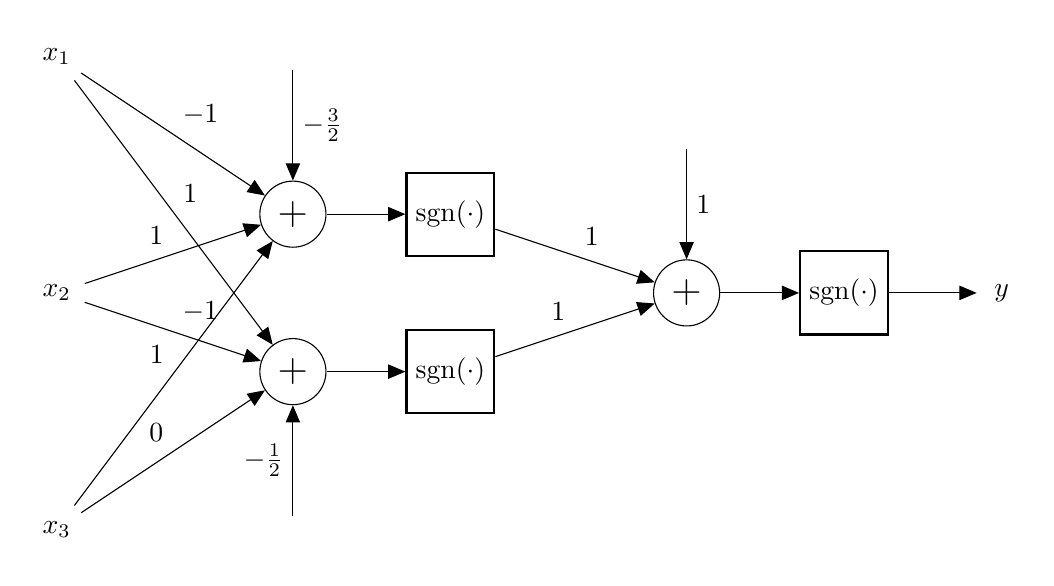
\begin{tikzpicture}[auto, node distance=2cm, >=triangle 45]

% Input layer
\draw node [input, name=x1] {$x_1$};
\draw node [input, name=x2, below of=x1, node distance=3cm] {$x_2$};
\draw node [input, name=x3, below of=x2, node distance=3cm] {$x_3$};

% First layer
\draw node [sum, right of=x2, yshift=1cm, node distance=3cm] (sum1) {\Large$+$};
\draw node [sum, below of=sum1] (sum2) {\Large$+$};
\draw node [input, name=x01, above of=sum1] {};
\draw node [input, name=x02, below of=sum2] {};
\draw node [block, right of=sum1] (act1) {sgn($\cdot$)};
\draw node [block, right of=sum2] (act2) {sgn($\cdot$)};

% Second layer
\draw node [sum, right of=act1, yshift=-1cm, node distance=3cm] (sum3) {\Large$+$};
\draw node [input, name=x03, above of=sum3] {};
\draw node [block, right of=sum3] (act3) {sgn($\cdot$)};
\draw node [output, name=y, right of=act3] {$y$};

% Connections
\draw[->](x01) -- node {$-\frac{3}{2}$}(sum1);
\draw[->](x1) -- node {$-1$}(sum1);
\draw[->](x2) -- node {$1$}(sum1);
\draw[->](x3) -- node {$1$}(sum1);
\draw[->](x02) -- node {$-\frac{1}{2}$}(sum2);
\draw[->](x1) -- node {$1$}(sum2);
\draw[->](x2) -- node {$-1$}(sum2);
\draw[->](x3) -- node {$0$}(sum2);
\draw[->](sum1) -- node {}(act1);
\draw[->](sum2) -- node {}(act2);
\draw[->](x03) -- node {$1$}(sum3);
\draw[->](act1) -- node {$1$}(sum3);
\draw[->](act2) -- node {$1$}(sum3);
\draw[->](sum3) -- node {}(act3);
\draw[->](act3) -- node {}(y);

\end{tikzpicture}
\caption{Final network that implements the given function}
\end{figure}

\section{Question 2}

\subsection{Analysis of the first layer}

In order to sketch the region in which the output of the network is $z = 1$, let's begin considering the first layer of neurons independently; for each of them, it is possible to write the input-output relationship, starting from the given weights:

\begin{itemize}

\item The first neuron implements the function $z_1 = u(1 + x - y)$, meaning that its output goes to 1 when $1 + x - y \ge 0 \Rightarrow y \le x + 1$;
\item The second neuron implements the function $z_2 = u(1 - x - y)$, meaning that its output goes to 1 when $1 - x - y \ge 0 \Rightarrow y \le -x + 1$;
\item The third neuron implements the function $z_3 = u(-x)$, meaning that its output goes to 1 when $-x \ge 0 \Rightarrow x \le 0$.

\end{itemize}

The regions in which the three neurons output a positive value can be represented on the $x$-$y$ plane as shown in the figure below.

\begin{figure}[h]
\centering
\includegraphics[width=\linewidth]{first_layer_out_sep.pdf}
\caption{Regions in which first layer neurons output a positive value}
\end{figure}

\subsection{Deduction of network output per region}

If we represent all those relationships on a single plane, then six different regions can be identified; each of those regions will represent a specific set of inputs of the second layer of the network. Analyzing those regions one by one, it is possible to deduce, for each of them, what will be the output of the network, given the input-output relationship of the second-layer neuron ($z = -1.5 + z_1 + z_2 - z_3$, where $z_1, z_2, z_3$ denote the outputs of the first-layer neurons):

\begin{enumerate}

\item In this region, the outputs of all first layer neurons is zero; therefore, the output $z$ of the neuron in the second layer is:

$$ z = u(-1.5 + 1 * 0 + 1 * 0 - 1 * 0) = u(-1.5) = 0 $$

\item In this region, the output of the first neuron is positive, while the outputs of the others are zero; therefore, the output $z$ of the neuron in the second layer is:

$$ z = u(-1.5 + 1 * 1 + 1 * 0 - 1 * 0) = u(-0.5) = 0 $$

\item In this region, the output of the first and second neurons are positive, while the output of the third is zero; therefore, the output $z$ of the neuron in the second layer is:

$$ z = u(-1.5 + 1 * 1 + 1 * 1 - 1 * 0) = u(0.5) = 1 $$

\item In this region, the outputs of all first layer neurons is positive; therefore, the output $z$ of the neuron in the second layer is:

$$ z = u(-1.5 + 1 * 1 + 1 * 1 - 1 * 1) = u(-0.5) = 0 $$

\item In this region, the output of the second and third neurons are positive, while the output of the first is zero; therefore, the output $z$ of the neuron in the second layer is:

$$ z = u(-1.5 + 1 * 0 + 1 * 1 - 1 * 1) = u(-1.5) = 0 $$

\item In this region, the output of the third neuron is positive, while the outputs of the others are zero; therefore, the output $z$ of the neuron in the second layer is:

$$ z = u(-1.5 + 1 * 0 + 1 * 0 - 1 * 1) = u(-2.5) = 0 $$

\end{enumerate}

\begin{figure}
\centering
\includegraphics[width=0.7\linewidth]{first_layer_out_all.pdf}
\caption{Combination of output regions of first layer neurons}
\end{figure}

The only region in which the network returns a positive value, therefore, is region number 3, including the separator of the second neuron (the blue line, on which the second neuron outputs $u(0) = 1$) but excluding the one of the third neuron (the green line, on which the third neuron outputs $u(0) = 1$). Graphically, it is possible to represent the two classes separated by this network on the $x$-$y$ plane as shown in the figure below; the dashed line indicates a zone for which $z = 0$, while the normal line a zone for which $z = 1$.

\begin{figure}[h]
\centering
\includegraphics[width=0.7\linewidth]{net_sep.pdf}
\caption{Classes separation using the given network}
\end{figure}

\section{Question 3}

\subsection{Complete Python code}

\lstinputlisting[basicstyle=\ttfamily\scriptsize,language=python]{hw1_ex3.py}

\end{document}